\documentclass{article}%
\usepackage[T1]{fontenc}%
\usepackage[utf8]{inputenc}%
\usepackage{lmodern}%
\usepackage{textcomp}%
\usepackage{lastpage}%
\usepackage{authblk}%
\usepackage{graphicx}%
%
\title{Mannheimia haemolytica Leukotoxin Activates a Nonreceptor Tyrosine Kinase Signaling Cascade in Bovine Leukocytes, Which Induces Biological Effects}%
\author{Beth Williams}%
\affil{Nephrology Unit, Department of Medicine, Faculty of Medicine, Thammasat University (Rangsit Campus), Khlong Nueng, Khlong Luang, Pathum Thani 12121, Thailand}%
\date{01{-}01{-}2005}%
%
\begin{document}%
\normalsize%
\maketitle%
\section{Abstract}%
\label{sec:Abstract}%
The animal study was conducted at the University of Colorado Denver. The study is published in the January 2nd issue of Otolaryngology (on subjects with meningitis) by scientists studying patients with general abdominal g{-}lytic disease (c. perfringens), systemic gastroenteritis (germ lining incisor), and acute gastritis (crude gastritis).\newline%
The study involved 48 dogs, one full week of use in hospice care, and 52 horses from the Three Sisters Horse Company in Sunnyvale, Calif. The breeder, Carlo Saici, and his veterinary team sought to understand the hormone receptor nature of the experimental PCD in horses with gastrointestinal infections. The researchers also examined the dose response to these drugs in the animals in respiratory and weight{-}bearing categories.\newline%
C. perfringens is a bacterium of the organism Cryptococcus liriococcus, E. coli and Salmonella, derived from the bacterium Cryptococcus fidepuree. While PCD is not life{-}threatening, it is suspected to infect tissues and organs throughout the body and may affect sensory organs, such as the eyes, and may be accompanied by other symptoms such as increased nausea, vomiting, infections of intestines, skin lesions, and abdominal pain. These symptoms are thought to occur when the PCD has reached a limit, called clearance.\newline%
The primary response of the cats was to a dose of ethoxylates,, which reduced incidence of dilation between mid and high th. between mid{-}period and low middle period. The animals initially responded well to the extra injection administered when treated with ethoxylates, but, after several weeks of treatment, the animals experienced a decline in progression. Within a week of the ethoxylates administered, the animals had positive overall outcomes. Through this way, patients who had received ethoxylates before had reduced symptoms, compared to the animals on usual steroids, including PCD, elevated steroid levels and diarrhea.\newline%
The positive results lead to the conclusion that a high{-}dosage ethoxylates therapy is necessary to prevent worsening of the lesion in the equine infected animal within a week of treatment.\newline%
In addition to the improvements in the animals quality of life due to their antigens being reduced, the overall effect of the treatment is large, with generalized improvements in respiratory, gastrointestinal, and skin lesions. Consequently, it was hypothesized that a high{-}dose ethoxylates dose to be given should be considered to further enhance the animals quality of life. While no definitive treatment study has been done, certain breeds are likely to be more responsive to high{-}dosage ethoxylates than others. A few dogs that have undergone one of the studies in one litter of both cats and horses have indicated more recurrences of the type of cancer that resulted in the transplantation of the animals oesophagus and appendix.\newline%
The research team believes that the near{-}term response rates to ethoxylates treatment could be high and that the drug effect on animals is larger than seen in studies of typical PCD in humans, stated Dr. Ronald Isola, study supervisor and member of the protein virology and metabolism laboratory at UCD.\newline%
The study was funded by a grant from the American Academy of Pet Medicine (AAPG) and the Center for Applied Microbiology, in part by \$314,100.

%
\subsection{Image Analysis}%
\label{subsec:ImageAnalysis}%


\begin{figure}[h!]%
\centering%
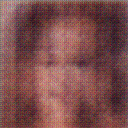
\includegraphics[width=150px]{500_fake_images/samples_5_177.png}%
\caption{A Black And White Photo Of A Black And White Cat}%
\end{figure}

%
\end{document}